\documentclass{standalone}
\usepackage{tikz}
\usetikzlibrary{patterns, positioning}

\begin{document}
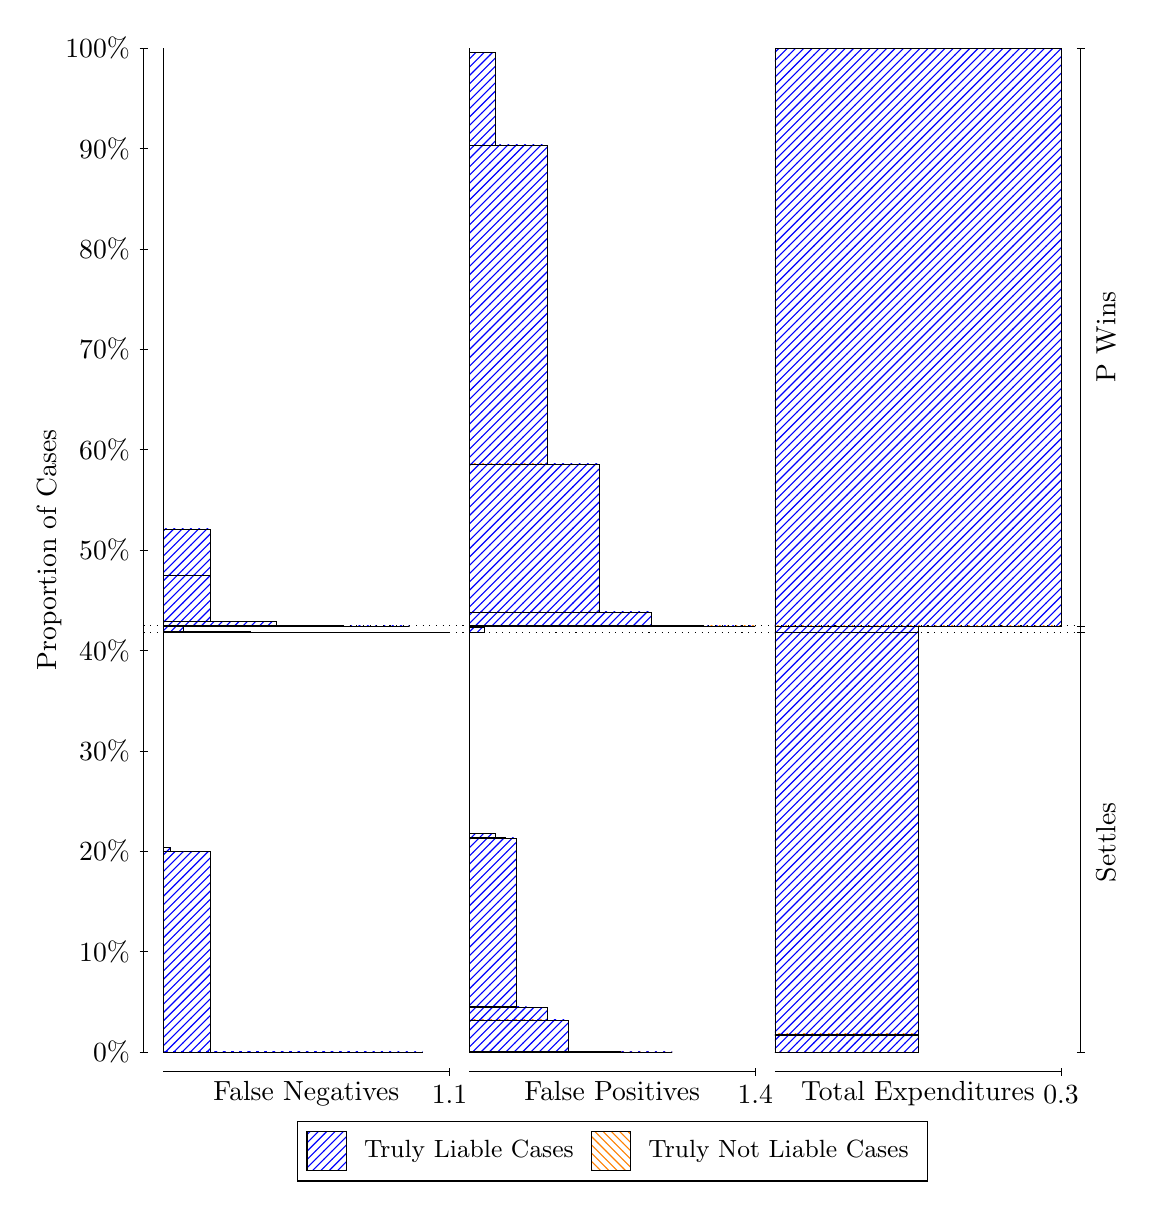
\begin{tikzpicture}
\draw[black, very thin] (1.5,1.75) -- (1.5,14.5);
\node[rotate=90, anchor=center] at (0.3, 8.125) {Proportion of Cases};
\draw[black, very thin] (1.45,1.75) -- (1.55,1.75);
\node[anchor=east] at (1.45, 1.75) {0\%};
\draw[black, very thin] (1.45,3.025) -- (1.55,3.025);
\node[anchor=east] at (1.45, 3.025) {10\%};
\draw[black, very thin] (1.45,4.3) -- (1.55,4.3);
\node[anchor=east] at (1.45, 4.3) {20\%};
\draw[black, very thin] (1.45,5.575) -- (1.55,5.575);
\node[anchor=east] at (1.45, 5.575) {30\%};
\draw[black, very thin] (1.45,6.85) -- (1.55,6.85);
\node[anchor=east] at (1.45, 6.85) {40\%};
\draw[black, very thin] (1.45,8.125) -- (1.55,8.125);
\node[anchor=east] at (1.45, 8.125) {50\%};
\draw[black, very thin] (1.45,9.4) -- (1.55,9.4);
\node[anchor=east] at (1.45, 9.4) {60\%};
\draw[black, very thin] (1.45,10.675) -- (1.55,10.675);
\node[anchor=east] at (1.45, 10.675) {70\%};
\draw[black, very thin] (1.45,11.95) -- (1.55,11.95);
\node[anchor=east] at (1.45, 11.95) {80\%};
\draw[black, very thin] (1.45,13.225) -- (1.55,13.225);
\node[anchor=east] at (1.45, 13.225) {90\%};
\draw[black, very thin] (1.45,14.5) -- (1.55,14.5);
\node[anchor=east] at (1.45, 14.5) {100\%};

\draw[black, very thin] (13.4,1.75) -- (13.4,14.5);
\draw[black, very thin] (13.35,1.75) -- (13.45,1.75);
\node[anchor=west] at (13.35, 1.75) {};
\draw[black, very thin] (13.35,7.0776) -- (13.45,7.0776);
\node[anchor=west] at (13.35, 7.0776) {};
\draw[black, very thin] (13.35,7.1625) -- (13.45,7.1625);
\node[anchor=west] at (13.35, 7.1625) {};
\draw[black, very thin] (13.35,14.5) -- (13.45,14.5);
\node[anchor=west] at (13.35, 14.5) {};

\draw[black, very thin, pattern color=blue, pattern=north east lines] (1.75,1.75) rectangle (5.0453,1.75);
\draw[black, very thin, pattern color=blue, pattern=north east lines] (1.75,1.75) rectangle (4.7074,1.75);
\draw[black, very thin, pattern color=blue, pattern=north east lines] (1.75,1.75) rectangle (4.3694,1.75);
\draw[black, very thin, pattern color=blue, pattern=north east lines] (1.75,1.75) rectangle (4.2004,1.75);
\draw[black, very thin, pattern color=blue, pattern=north east lines] (1.75,1.75) rectangle (4.0314,1.75);
\draw[black, very thin, pattern color=blue, pattern=north east lines] (1.75,1.75) rectangle (3.8624,1.75);
\draw[black, very thin, pattern color=blue, pattern=north east lines] (1.75,1.75) rectangle (3.6934,1.75);
\draw[black, very thin, pattern color=blue, pattern=north east lines] (1.75,1.75) rectangle (3.5244,1.75);
\draw[black, very thin, pattern color=blue, pattern=north east lines] (1.75,1.75) rectangle (3.3554,1.75);
\draw[black, very thin, pattern color=blue, pattern=north east lines] (1.75,1.75) rectangle (3.1864,1.75);
\draw[black, very thin, pattern color=blue, pattern=north east lines] (1.75,1.75) rectangle (3.1864,1.75);
\draw[black, very thin, pattern color=blue, pattern=north east lines] (1.75,1.75) rectangle (3.0174,1.75);
\draw[black, very thin, pattern color=blue, pattern=north east lines] (1.75,1.75) rectangle (2.8484,1.75);
\draw[black, very thin, pattern color=blue, pattern=north east lines] (1.75,1.75) rectangle (2.6795,1.7504);
\draw[black, very thin, pattern color=blue, pattern=north east lines] (1.75,1.7504) rectangle (2.6795,1.7504);
\draw[black, very thin, pattern color=blue, pattern=north east lines] (1.75,1.7504) rectangle (2.5105,1.7519);
\draw[black, very thin, pattern color=blue, pattern=north east lines] (1.75,1.7519) rectangle (2.3415,1.7519);
\draw[black, very thin, pattern color=blue, pattern=north east lines] (1.75,1.7519) rectangle (2.3415,1.752);
\draw[black, very thin, pattern color=blue, pattern=north east lines] (1.75,1.752) rectangle (2.3415,4.2978);
\draw[black, very thin, pattern color=blue, pattern=north east lines] (1.75,4.2978) rectangle (2.1725,4.2992);
\draw[black, very thin, pattern color=blue, pattern=north east lines] (1.75,4.2992) rectangle (2.0035,4.2992);
\draw[black, very thin, pattern color=blue, pattern=north east lines] (1.75,4.2992) rectangle (1.8345,4.3476);
\draw[black, very thin, pattern color=blue, pattern=north east lines] (1.75,4.3476) rectangle (1.8345,4.3476);
\draw[black, very thin, pattern color=orange, pattern=north west lines] (1.75,4.3476) rectangle (1.75,4.3476);
\draw[black, very thin, pattern color=blue, pattern=north east lines] (1.75,4.3476) rectangle (1.75,7.0776);
\draw[black, very thin, pattern color=blue, pattern=north east lines] (1.75,7.0776) rectangle (5.3833,7.0776);
\draw[black, very thin, pattern color=blue, pattern=north east lines] (1.75,7.0776) rectangle (4.5384,7.0776);
\draw[black, very thin, pattern color=blue, pattern=north east lines] (1.75,7.0776) rectangle (3.6934,7.0777);
\draw[black, very thin, pattern color=blue, pattern=north east lines] (1.75,7.0777) rectangle (2.8484,7.0902);
\draw[black, very thin, pattern color=blue, pattern=north east lines] (1.75,7.0902) rectangle (2.0035,7.1625);
\draw[black, very thin, pattern color=orange, pattern=north west lines] (1.75,7.1625) rectangle (1.75,7.1625);
\draw[black, very thin, pattern color=blue, pattern=north east lines] (1.75,7.1625) rectangle (4.8764,7.1625);
\draw[black, very thin, pattern color=blue, pattern=north east lines] (1.75,7.1625) rectangle (4.0314,7.1627);
\draw[black, very thin, pattern color=blue, pattern=north east lines] (1.75,7.1627) rectangle (3.1864,7.22);
\draw[black, very thin, pattern color=blue, pattern=north east lines] (1.75,7.22) rectangle (2.3415,7.8097);
\draw[black, very thin, pattern color=blue, pattern=north east lines] (1.75,7.8097) rectangle (2.3415,8.3925);
\draw[black, very thin, pattern color=orange, pattern=north west lines] (1.75,8.3925) rectangle (1.75,8.3925);
\draw[black, very thin, pattern color=blue, pattern=north east lines] (1.75,8.3925) rectangle (1.75,14.5);
\draw[black, very thin, pattern color=orange, pattern=north west lines] (5.6333,1.75) rectangle (8.2097,1.75);
\draw[black, very thin, pattern color=blue, pattern=north east lines] (5.6333,1.75) rectangle (8.2097,1.75);
\draw[black, very thin, pattern color=orange, pattern=north west lines] (5.6333,1.75) rectangle (7.9455,1.75);
\draw[black, very thin, pattern color=blue, pattern=north east lines] (5.6333,1.75) rectangle (7.9455,1.75);
\draw[black, very thin, pattern color=orange, pattern=north west lines] (5.6333,1.75) rectangle (7.6812,1.75);
\draw[black, very thin, pattern color=blue, pattern=north east lines] (5.6333,1.75) rectangle (7.6812,1.75);
\draw[black, very thin, pattern color=blue, pattern=north east lines] (5.6333,1.75) rectangle (7.5491,1.7532);
\draw[black, very thin, pattern color=orange, pattern=north west lines] (5.6333,1.7532) rectangle (7.417,1.7532);
\draw[black, very thin, pattern color=blue, pattern=north east lines] (5.6333,1.7532) rectangle (7.417,1.7532);
\draw[black, very thin, pattern color=blue, pattern=north east lines] (5.6333,1.7532) rectangle (7.2848,1.7532);
\draw[black, very thin, pattern color=orange, pattern=north west lines] (5.6333,1.7532) rectangle (7.1527,1.7532);
\draw[black, very thin, pattern color=blue, pattern=north east lines] (5.6333,1.7532) rectangle (7.1527,1.7533);
\draw[black, very thin, pattern color=blue, pattern=north east lines] (5.6333,1.7533) rectangle (7.0206,1.7534);
\draw[black, very thin, pattern color=orange, pattern=north west lines] (5.6333,1.7534) rectangle (6.8885,1.7534);
\draw[black, very thin, pattern color=blue, pattern=north east lines] (5.6333,1.7534) rectangle (6.8885,1.7536);
\draw[black, very thin, pattern color=orange, pattern=north west lines] (5.6333,1.7536) rectangle (6.8885,1.7536);
\draw[black, very thin, pattern color=blue, pattern=north east lines] (5.6333,1.7536) rectangle (6.8885,2.1579);
\draw[black, very thin, pattern color=blue, pattern=north east lines] (5.6333,2.1579) rectangle (6.7564,2.1581);
\draw[black, very thin, pattern color=orange, pattern=north west lines] (5.6333,2.1581) rectangle (6.6242,2.1581);
\draw[black, very thin, pattern color=blue, pattern=north east lines] (5.6333,2.1581) rectangle (6.6242,2.3158);
\draw[black, very thin, pattern color=blue, pattern=north east lines] (5.6333,2.3158) rectangle (6.4921,2.3172);
\draw[black, very thin, pattern color=orange, pattern=north west lines] (5.6333,2.3172) rectangle (6.36,2.3172);
\draw[black, very thin, pattern color=blue, pattern=north east lines] (5.6333,2.3172) rectangle (6.36,2.3217);
\draw[black, very thin, pattern color=blue, pattern=north east lines] (5.6333,2.3217) rectangle (6.36,2.3218);
\draw[black, very thin, pattern color=blue, pattern=north east lines] (5.6333,2.3218) rectangle (6.2279,2.3242);
\draw[black, very thin, pattern color=blue, pattern=north east lines] (5.6333,2.3242) rectangle (6.2279,4.4691);
\draw[black, very thin, pattern color=orange, pattern=north west lines] (5.6333,4.4691) rectangle (6.0958,4.4691);
\draw[black, very thin, pattern color=blue, pattern=north east lines] (5.6333,4.4691) rectangle (6.0958,4.4799);
\draw[black, very thin, pattern color=blue, pattern=north east lines] (5.6333,4.4799) rectangle (6.0958,4.4801);
\draw[black, very thin, pattern color=blue, pattern=north east lines] (5.6333,4.4801) rectangle (5.9636,4.5284);
\draw[black, very thin, pattern color=blue, pattern=north east lines] (5.6333,4.5284) rectangle (5.8315,4.5285);
\draw[black, very thin, pattern color=blue, pattern=north east lines] (5.6333,4.5285) rectangle (5.6994,4.5299);
\draw[black, very thin, pattern color=blue, pattern=north east lines] (5.6333,4.5299) rectangle (5.6994,4.5299);
\draw[black, very thin, pattern color=blue, pattern=north east lines] (5.6333,4.5299) rectangle (5.6333,7.0776);
\draw[black, very thin, pattern color=orange, pattern=north west lines] (5.6333,7.0776) rectangle (5.8315,7.0776);
\draw[black, very thin, pattern color=blue, pattern=north east lines] (5.6333,7.0776) rectangle (5.8315,7.1499);
\draw[black, very thin, pattern color=blue, pattern=north east lines] (5.6333,7.1499) rectangle (5.6333,7.1625);
\draw[black, very thin, pattern color=orange, pattern=north west lines] (5.6333,7.1625) rectangle (9.2667,7.1625);
\draw[black, very thin, pattern color=blue, pattern=north east lines] (5.6333,7.1625) rectangle (9.2667,7.1625);
\draw[black, very thin, pattern color=orange, pattern=north west lines] (5.6333,7.1625) rectangle (8.6061,7.1625);
\draw[black, very thin, pattern color=blue, pattern=north east lines] (5.6333,7.1625) rectangle (8.6061,7.1649);
\draw[black, very thin, pattern color=orange, pattern=north west lines] (5.6333,7.1649) rectangle (7.9455,7.1649);
\draw[black, very thin, pattern color=blue, pattern=north east lines] (5.6333,7.1649) rectangle (7.9455,7.3383);
\draw[black, very thin, pattern color=orange, pattern=north west lines] (5.6333,7.3383) rectangle (7.2848,7.3383);
\draw[black, very thin, pattern color=blue, pattern=north east lines] (5.6333,7.3383) rectangle (7.2848,9.2177);
\draw[black, very thin, pattern color=orange, pattern=north west lines] (5.6333,9.2177) rectangle (6.6242,9.2177);
\draw[black, very thin, pattern color=blue, pattern=north east lines] (5.6333,9.2177) rectangle (6.6242,13.27);
\draw[black, very thin, pattern color=blue, pattern=north east lines] (5.6333,13.27) rectangle (5.9636,14.443);
\draw[black, very thin, pattern color=blue, pattern=north east lines] (5.6333,14.443) rectangle (5.6333,14.5);
\draw[black, very thin, pattern color=orange, pattern=north west lines] (9.5167,1.75) rectangle (11.333,1.75);
\draw[black, very thin, pattern color=blue, pattern=north east lines] (9.5167,1.75) rectangle (11.333,1.965);
\draw[black, very thin, pattern color=orange, pattern=north west lines] (9.5167,1.965) rectangle (11.333,1.965);
\draw[black, very thin, pattern color=blue, pattern=north east lines] (9.5167,1.965) rectangle (11.333,1.9788);
\draw[black, very thin, pattern color=orange, pattern=north west lines] (9.5167,1.9788) rectangle (11.333,1.9788);
\draw[black, very thin, pattern color=blue, pattern=north east lines] (9.5167,1.9788) rectangle (11.333,7.0776);
\draw[black, very thin, pattern color=orange, pattern=north west lines] (9.5167,7.0776) rectangle (11.333,7.0776);
\draw[black, very thin, pattern color=blue, pattern=north east lines] (9.5167,7.0776) rectangle (11.333,7.1625);
\draw[black, very thin, pattern color=orange, pattern=north west lines] (9.5167,7.1625) rectangle (13.15,7.1625);
\draw[black, very thin, pattern color=blue, pattern=north east lines] (9.5167,7.1625) rectangle (13.15,14.5);
\draw[black, dotted] (1.5,7.0776) -- (13.4,7.0776);
\draw[black, dotted] (1.5,7.1625) -- (13.4,7.1625);
\draw[black, very thin] (1.75,1.5) -- (5.3833,1.5);
\node[anchor=north] at (3.5667, 1.5) {False Negatives};
\draw[black, very thin] (5.3833,1.45) -- (5.3833,1.55);
\node[anchor=north] at (5.3833, 1.45) {1.1};

\draw[black, very thin] (5.6333,1.5) -- (9.2667,1.5);
\node[anchor=north] at (7.45, 1.5) {False Positives};
\draw[black, very thin] (9.2667,1.45) -- (9.2667,1.55);
\node[anchor=north] at (9.2667, 1.45) {1.4};

\draw[black, very thin] (9.5167,1.5) -- (13.15,1.5);
\node[anchor=north] at (11.333, 1.5) {Total Expenditures};
\draw[black, very thin] (13.15,1.45) -- (13.15,1.55);
\node[anchor=north] at (13.15, 1.45) {0.3};

\node[black, centered, rotate=90] at (13.72, 4.4138) {Settles};

\node[black, centered, rotate=90] at (13.72, 10.831) {P Wins};

\draw (7.449999999999999,1.5) node[draw=none] (baseCoordinate) {};
\begin{scope}[align=center]
        \matrix[scale=0.5, draw=black, below=0.5cm of baseCoordinate, nodes={draw}, column sep=0.1cm]{
            \node[rectangle, draw, minimum width=0.5cm, minimum height=0.5cm, pattern=north east lines, pattern color=blue] {}; &
            \node[draw=none, font=\small] (B) {Truly Liable Cases}; &
            \node[rectangle, draw, minimum width=0.5cm, minimum height=0.5cm, pattern=north west lines, pattern color=orange] {}; &
            \node[draw=none, font=\small] (B) {Truly Not Liable Cases}; \\
            };
\end{scope}

\end{tikzpicture}
\end{document}